% FYS-STK3155 Project 2. Compile with
%   pdflatex main && bibtex main && pdflatex main && pdflatex main
% Figures are read from ../Code/figures/. Every number in the text is taken
% from the logs in ../Code/results/ (part_b.txt ... part_e.txt).
\documentclass[english,notitlepage,reprint,nofootinbib,floatfix]{revtex4-1}
\usepackage[utf8]{inputenc}
\usepackage[T1]{fontenc}
\usepackage{mathpazo}
\usepackage{amsmath,amssymb}
\usepackage{graphicx}
\usepackage{booktabs}
\usepackage{listings}
\usepackage{xcolor}
\usepackage[ruled,linesnumbered]{algorithm2e}
\usepackage[colorlinks=true,linkcolor=blue,citecolor=blue,urlcolor=blue]{hyperref}
\graphicspath{{../Code/figures/}}

% No paragraph indentation; a small space between paragraphs instead
\setlength{\parindent}{0pt}
\setlength{\parskip}{0.5\baselineskip plus 2pt minus 1pt}

% Terminal-style blocks for program output
\definecolor{termBg}{HTML}{0C0C0C}
\definecolor{termText}{HTML}{CCCCCC}
\lstdefinestyle{terminal}{
  backgroundcolor=\color{termBg},
  basicstyle=\ttfamily\scriptsize\color{termText},
  columns=flexible, keepspaces=true,
  breaklines=true, showstringspaces=false, frame=none,
  xleftmargin=4pt, xrightmargin=4pt,
  framexleftmargin=4pt, framexrightmargin=4pt,
  framextopmargin=4pt, framexbottommargin=4pt,
}

\begin{document}
\title{Regression and classification with a feed-forward neural network written from scratch}
\author{andreand}
% \author{suadrn}
\affiliation{University of Oslo}
\date{\today}

\begin{abstract}
We wrote our own feed-forward neural network with backpropagation, checked it against automatic differentiation and against ordinary least squares (OLS), and used it for regression on the noisy Runge function of Project 1 and for classification of the MNIST handwritten digits. One hidden layer of 50 sigmoid nodes was not better than OLS of degree 12: over ten data sets the median test MSE was 0.0132 against 0.0122. A ReLU network with three hidden layers of 50 nodes and a small learning rate gave 0.0093 on the 20 data sets of Project 1, against 0.0133 for Ridge, close to the noise level of 0.0091. $L_1$ and $L_2$ penalties gave no measurable improvement. Plain gradient descent needed a learning rate 100 times larger than RMSprop and Adam, and converged more slowly. On MNIST, one hidden layer of 200 ReLU nodes gave a test accuracy of 97.8\,\%, against 92.7\,\% for logistic regression, our network without hidden layers, and most of the remaining errors were between digits that can look alike, such as 4 and 9.
\end{abstract}

\maketitle

% =====================================================================
% INTRODUCTION
% LLM declaration: text level 3; see the appendix "Use of AI/LLM tools".
% =====================================================================

\section*{Introduction}

In Project 1 we fitted polynomials to noisy samples of Runge's function, $f(x) = 1/(1 + 25x^2)$ \cite{Runge1901}. The features, the powers $x, x^2, \dots, x^d$, were chosen by us, and the best degree had to be found by testing. A neural network takes the raw input and learns its own features in the hidden layers. The universal approximation theorem says that one hidden layer with enough nodes can approximate any continuous function on a bounded interval as well as we want \cite[Sec.~8.4]{HjorthJensen2026}, but not how to find the weights, or how much data that takes.

We wrote our own feed-forward neural network (FFNN) with backpropagation. It has a flexible number of layers and nodes, a choice of activation function in each layer (sigmoid, ReLU, Leaky ReLU, linear and softmax), the mean squared error or the cross entropy as cost function, and optional $L_1$ or $L_2$ penalties on the weights. It is trained with the gradient-descent code from Project 1: plain gradient descent, and stochastic gradient descent with RMSprop or Adam.

For regression we used the data sets of Runge's function from Project 1, and compared with the OLS, Ridge and Lasso results there. For classification we used the MNIST data set of handwritten digits \cite{LeCun2010MNIST}, and compared with logistic regression, which is our network without hidden layers, and with scikit-learn \cite{Pedregosa2011}.

The Methods section describes the cost functions and their gradients (part a of the project), the network, backpropagation, the initialisation, the optimisers, the data and how we tested the code. The Results and discussion section follows parts b--e, the Critical evaluation section compares the methods (part f), and the Conclusion sums up. We used NumPy \cite{Harris2020}, JAX \cite{Jax2018} to check our gradients, scikit-learn for splitting data and as a reference, and Matplotlib \cite{Hunter2007} for the figures. The code, the logged output and the figures are on GitHub\footnote{\url{https://github.com/mrleenudler/FYS-STK3155/tree/main/project_2}}.

% =====================================================================
% METHODS
% LLM declaration: text level 3; see the appendix "Use of AI/LLM tools".
% =====================================================================

\section*{Methods}

\subsection*{Data}

\emph{Runge's function.} As in Project 1, $x$ was drawn uniformly from $[-1, 1]$ and $y_i = f(x_i) + \varepsilon_i$ with $\varepsilon_i \sim \mathcal{N}(0, \sigma^2)$, $n = 100$ and $\sigma = 0.1$. One seed fixes the data and the 80/20 split into training and test points, with the code from Project 1, so seed 42 gives the same data set as there. To choose the hyperparameters we split the 80 training points into 64 for training and 16 for validation, and the test points were used only for the final comparisons. The input to the network is $x$ alone, standardised with the mean and standard deviation of the training points. The targets were not scaled, since the output layer has a bias.

\emph{MNIST.} The data set has $70\,000$ grey-scale images of $28 \times 28$ pixels, with a canonical split into $60\,000$ training and $10\,000$ test images \cite{LeCun2010MNIST}. We drew $10\,000$ of the training images at random (seed 2026) as a validation set for all choices of hyperparameters, trained on the other $50\,000$, and used the test set once, at the end. The images were flattened to 784 pixel values, which were divided by 255 so that they lie in $[0, 1]$, and the targets are one-hot vectors with ten components.

\subsection*{The network}

As in the lecture notes \cite[Sec.~8.5]{HjorthJensen2026} and the exercises of weeks 41 and 42, the samples are the rows of the input $\mathbf{X}$, and layer $l$ has a weight matrix $\mathbf{W}^l$ of shape (inputs, outputs) and a bias vector $\mathbf{b}^l$. The feed-forward pass is
$$
\mathbf{z}^l = \mathbf{a}^{l-1}\mathbf{W}^l + \mathbf{b}^l, \qquad \mathbf{a}^l = f^l(\mathbf{z}^l), \qquad l = 1, \dots, L,
$$
with $\mathbf{a}^0 = \mathbf{X}$. Here $\mathbf{z}^l$ and $\mathbf{a}^l$ have one row per sample, the bias is added to every row, and the activation function $f^l$ acts on each element (the softmax on each row).

\subsection*{Cost functions and their gradients}

\emph{Mean squared error.} For the regression, with one output node, we used the cost from Project 1,
$$
C_{\mathrm{MSE}} = \frac{1}{n}\sum_{i=1}^{n}(a_i - y_i)^2, \qquad \frac{\partial C_{\mathrm{MSE}}}{\partial a_i} = \frac{2}{n}(a_i - y_i),
$$
where $a_i$ is the output for sample $i$ and $y_i$ the target.

\emph{Binary cross entropy.} For two classes the output is one sigmoid node, $a_i = \sigma(z_i)$, the probability that $y_i = 1$, and
$$
C_{\mathrm{BCE}} = -\frac{1}{n}\sum_{i=1}^{n}\left[y_i\ln a_i + (1 - y_i)\ln(1 - a_i)\right].
$$
For $y_i = 1$ only the first term counts, and $-\ln a_i$ grows without limit as $a_i \to 0$, so a confident wrong answer costs a lot; the second term does the same for $y_i = 0$. The cost is the negative log-likelihood of the targets \cite[Sec.~5.3]{HjorthJensen2026}. Its derivative is
$$
\frac{\partial C_{\mathrm{BCE}}}{\partial a_i} = \frac{1}{n}\left(-\frac{y_i}{a_i} + \frac{1 - y_i}{1 - a_i}\right) = \frac{1}{n}\,\frac{a_i - y_i}{a_i(1 - a_i)},
$$
and since $\sigma'(z) = \sigma(z)\left(1 - \sigma(z)\right) = a(1 - a)$,
$$
\frac{\partial C_{\mathrm{BCE}}}{\partial z_i} = \frac{1}{n}(a_i - y_i).
$$

\emph{Multiclass cross entropy.} For $K$ classes the output layer has $K$ softmax nodes, and the targets are one-hot, $y_{ik} = 1$ for the correct class and 0 for the others \cite[Sec.~5.6]{HjorthJensen2026}:
$$
a_{ik} = \frac{e^{z_{ik}}}{\sum_{j=1}^{K} e^{z_{ij}}}, \qquad C_{\mathrm{CE}} = -\frac{1}{n}\sum_{i=1}^{n}\sum_{k=1}^{K} y_{ik}\ln a_{ik}.
$$
The softmax gives positive outputs that sum to one, and the cost is the average of $-\ln$ of the probability given to the correct class. Since
$$
\ln a_{ik} = z_{ik} - \ln\sum_{j=1}^{K} e^{z_{ij}},
$$
the derivative is
$$
\frac{\partial C_{\mathrm{CE}}}{\partial z_{ik}} = \frac{1}{n}\left(-y_{ik} + a_{ik}\sum_{m=1}^{K} y_{im}\right) = \frac{1}{n}(a_{ik} - y_{ik}),
$$
since the one-hot targets of a sample sum to one.

\emph{Matched pairs.} The linear output with the MSE, the sigmoid with the binary cross entropy and the softmax with the cross entropy thus give the same form of output error,
$$
\boldsymbol{\delta}^L = \frac{\partial C}{\partial \mathbf{z}^L} = c\,(\mathbf{a}^L - \mathbf{y}),
$$
with $c = 2/n$ for the MSE and $c = 1/n$ for the cross entropies. With a mixed pair, for instance a sigmoid output with the MSE, the factor $\sigma'(z^L)$ stays in $\boldsymbol{\delta}^L$. It is close to zero when the output saturates, also when the output is confidently wrong, so the network learns slowly exactly where it should learn the most.

\emph{Penalties.} With an $L_2$ or an $L_1$ penalty the cost becomes
$$
C = C_{\mathrm{data}} + \lambda\sum_{l}\sum_{j,k}\left(w^l_{jk}\right)^2 \qquad (L_2),
$$
$$
C = C_{\mathrm{data}} + \lambda\sum_{l}\sum_{j,k}\left|w^l_{jk}\right| \qquad (L_1),
$$
where $C_{\mathrm{data}}$ is one of the three costs above and the sums go over all weights in all layers. The penalty pulls the weights towards zero, and $\lambda \ge 0$ sets how hard. As for the intercept in Project 1, the biases are not penalised \cite[Sec.~8.12]{HjorthJensen2026}. The penalty depends on the weights directly and not through $\mathbf{z}^l$, so $\boldsymbol{\delta}^l$ is unchanged, and the weight gradient just gets an extra term,
$$
\frac{\partial C}{\partial \mathbf{W}^l} = \frac{\partial C_{\mathrm{data}}}{\partial \mathbf{W}^l} + 2\lambda\mathbf{W}^l \qquad (L_2),
$$
$$
\frac{\partial C}{\partial \mathbf{W}^l} = \frac{\partial C_{\mathrm{data}}}{\partial \mathbf{W}^l} + \lambda\,\mathrm{sign}(\mathbf{W}^l) \qquad (L_1),
$$
for all three costs. The absolute value has no derivative at zero, and as in Project 1 we used the subgradient with $\mathrm{sign}(0) = 0$. For the results we used the MSE and the multiclass cross entropy; the binary cross entropy is implemented and tested, but not used.

\subsection*{Activation functions}

For the hidden layers we used \cite[Sec.~8.6]{HjorthJensen2026}
$$
\sigma(z) = \frac{1}{1 + e^{-z}}, \qquad \sigma'(z) = \sigma(z)\left(1 - \sigma(z)\right),
$$
$$
\mathrm{ReLU}(z) = \max(0, z), \qquad \mathrm{ReLU}'(z) = \begin{cases} 1, & z > 0, \\ 0, & z \le 0, \end{cases}
$$
$$
\mathrm{LReLU}(z) = \begin{cases} z, & z > 0, \\ \alpha z, & z \le 0, \end{cases} \quad\; \mathrm{LReLU}'(z) = \begin{cases} 1, & z > 0, \\ \alpha, & z \le 0, \end{cases}
$$
with $\alpha = 0.01$. The derivative of the sigmoid is at most $1/4$, at $z = 0$, and goes to zero for large $|z|$, where the node saturates. ReLU does not saturate for $z > 0$, but a node with $z \le 0$ for all inputs gets no gradient and stops learning, a dead node. Leaky ReLU keeps the slope $\alpha$ for $z \le 0$, so its gradient is never zero. At $z = 0$, where ReLU has no derivative, we used 0. The output layer is linear, $f(z) = z$, for the regression, and the softmax for the classification.

\subsection*{Backpropagation}

The gradient with respect to all weights and biases follows from the chain rule, organised as the four equations of backpropagation \cite[Sec.~8.8.4]{HjorthJensen2026}. With $\boldsymbol{\delta}^l = \partial C / \partial \mathbf{z}^l$, one row per sample, they read in our batch form
$$
\boldsymbol{\delta}^L = f'(\mathbf{z}^L)\odot\frac{\partial C}{\partial \mathbf{a}^L}, \qquad
\boldsymbol{\delta}^l = \left(\boldsymbol{\delta}^{l+1}\left(\mathbf{W}^{l+1}\right)^T\right)\odot f'(\mathbf{z}^l),
$$
$$
\frac{\partial C}{\partial \mathbf{W}^l} = \left(\mathbf{a}^{l-1}\right)^T\boldsymbol{\delta}^l, \qquad
\frac{\partial C}{\partial \mathbf{b}^l} = \sum_{i=1}^{n}\boldsymbol{\delta}^l_{i},
$$
where $\odot$ is the element-wise product and $\boldsymbol{\delta}^l_i$ is row $i$ of $\boldsymbol{\delta}^l$. For the matched pairs the first equation is replaced by $\boldsymbol{\delta}^L = c\,(\mathbf{a}^L - \mathbf{y})$. The product $(\mathbf{a}^{l-1})^T\boldsymbol{\delta}^l$ sums over the samples; for one sample it is the outer product of the input to the layer and its error. The forward pass stores $\mathbf{a}^{l-1}$ and $\mathbf{z}^l$ for every layer, and one backward pass then gives all the gradients. The backward pass needs about as many operations as the forward pass, so the whole gradient costs roughly two forward passes, whatever the number of parameters. This is reverse-mode automatic differentiation applied to a layered function \cite[Secs.~4.14, 8.8]{HjorthJensen2026}. Algorithm~\ref{alg:train} shows the training loop.

\begin{algorithm}
\caption{Training with minibatches}\label{alg:train}
initialise $\mathbf{W}^l$ and $\mathbf{b}^l$ for $l = 1, \dots, L$\;
\For{each epoch}{
    shuffle the rows of the training data\;
    \For{each minibatch $(\mathbf{X}_B, \mathbf{y}_B)$}{
        forward pass from $\mathbf{a}^0 = \mathbf{X}_B$, storing $\mathbf{a}^{l-1}$ and $\mathbf{z}^l$\;
        $\boldsymbol{\delta}^L = c\,(\mathbf{a}^L - \mathbf{y}_B)$\;
        \For{$l = L, \dots, 1$}{
            $\partial C/\partial\mathbf{W}^l = (\mathbf{a}^{l-1})^T\boldsymbol{\delta}^l$ $+$ penalty term\;
            $\partial C/\partial\mathbf{b}^l = \sum_i \boldsymbol{\delta}^l_i$\;
            \lIf{$l > 1$}{$\boldsymbol{\delta}^{l-1} = \left(\boldsymbol{\delta}^l(\mathbf{W}^l)^T\right)\odot f'(\mathbf{z}^{l-1})$}
        }
        update every $\mathbf{W}^l$ and $\mathbf{b}^l$ with the optimiser\;
    }
}
\end{algorithm}

\subsection*{Initialisation}

The weights were drawn from a normal distribution with mean zero and a variance that depends on the number of inputs $n_{\mathrm{in}}$ to the layer \cite[Sec.~8.10]{HjorthJensen2026}. Since $z = \sum_i w_i a_i$ is a sum of $n_{\mathrm{in}}$ independent terms,
$$
\mathrm{Var}(z) = n_{\mathrm{in}}\,\mathrm{Var}(w)\,\mathrm{Var}(a),
$$
and $\mathrm{Var}(w) = 1/n_{\mathrm{in}}$ keeps the variance the same from layer to layer \cite{Glorot2010}. With too small weights the signal dies out, and with too large weights the sigmoid saturates. We used this for the sigmoid layers and for the linear and softmax output layers, as in Sec.~8.13 of the lecture notes, and $\mathrm{Var}(w) = 2/n_{\mathrm{in}}$ for ReLU and Leaky ReLU, which set about half of their inputs to zero \cite{He2015}. The weights must also start at different values, since equal weights give equal nodes that stay equal. The biases were set to 0.01 \cite[Sec.~8.10]{HjorthJensen2026}.

\subsection*{Optimisers}

We reused the update rules of Project 1 unchanged \cite[Secs.~4.7, 4.10, 4.11]{HjorthJensen2026}, and every element of every weight matrix and bias vector is updated with its own memory. With $g$ the gradient of a parameter $\theta$, plain gradient descent takes the step
$$
\theta \leftarrow \theta - \gamma g .
$$
RMSprop keeps a running average of the squared gradient and divides by its square root,
$$
s \leftarrow \rho s + (1 - \rho)g^2, \qquad \theta \leftarrow \theta - \gamma\,\frac{g}{\sqrt{s} + \epsilon},
$$
with $\rho = 0.99$ and $\epsilon = 10^{-8}$. Adam \cite{Kingma2015} does the same with $\beta_2 = 0.999$ in place of $\rho$, and also replaces $g$ by the running average
$$
m \leftarrow \beta_1 m + (1 - \beta_1)g
$$
with $\beta_1 = 0.9$, which works like momentum; both averages are corrected for starting at zero. Because of the division by $\sqrt{s}$, every parameter takes steps of about the size $\gamma$ in RMSprop and Adam, whether its gradient is large or small, while the step of plain gradient descent is $\gamma$ times the gradient.

In stochastic gradient descent (SGD) the gradient is computed on a minibatch. The rows of the training data are shuffled at the start of every epoch and gone through in minibatches of 16 rows (Runge) or 128 rows (MNIST), so an epoch is one pass through the training data. Plain gradient descent (GD) uses all the training data in every step: with 64 training points GD makes one update per epoch, and SGD with minibatches of 16 makes four. We trained for a fixed number of epochs, 1000 for Runge and 20 for MNIST, and stopped earlier only if a parameter became infinite or not a number.

\subsection*{Choice of hyperparameters}

The learning rate $\gamma$, the penalty $\lambda$, the number of hidden layers and nodes, and the activation function were chosen on the validation data, two at a time in grids shown as heat maps. For Runge the validation set has only 16 points. The MSE on 16 points is a mean of 16 squared errors, and its standard error, the standard deviation of the squared errors divided by $\sqrt{16}$ \cite[Eq.~2.24]{HjorthJensen2026}, was 18--34\,\% of the MSE for the two models we checked (OLS of degree 12 and a ReLU network, seeds 42--44). In parts c and d we therefore report the median validation MSE over three data sets, seeds 42, 43 and 44, with new data, split and initial weights each time. For MNIST the validation set has $10\,000$ images, and the standard error of an accuracy $p$ is $\sqrt{p(1 - p)/n} = 0.0014$ at $p = 0.98$.

\subsection*{Benchmarks and measures}

In part b we compared with OLS of degree 12 on the seed-42 split, the degree with the lowest test MSE for that split in Project 1 (0.0086). In part d we compared with the final models of Project 1: OLS, Ridge and Lasso with the degree and $\lambda$ chosen by 5-fold cross-validation on the training part of each of 20 data sets (seeds 42--61). Since we know $f$, we also computed the mean squared noise $(y_i - f(x_i))^2$ in the test sets, which is the test MSE of the true function itself.

For the classification the baseline is logistic regression, our network with no hidden layer, trained with the same code. An even simpler reference is to always guess the most common digit. We also compared with scikit-learn \cite{Pedregosa2011}: \texttt{LogisticRegression} with its default settings, which include an $L_2$ penalty, and \texttt{MLPClassifier} with the same hidden layer, optimiser, learning rate, minibatch size and number of epochs as our network, and no penalty.

The accuracy is the share of correctly classified images. In the confusion matrix, element $(i, j)$ is the number of test images of digit $i$ classified as $j$. The precision of digit $k$ is the share of the images classified as $k$ that really are $k$ (diagonal element over column sum), and the recall is the share of the images of $k$ classified as $k$ (diagonal element over row sum) \cite[Sec.~5.12]{HjorthJensen2026}.

\subsection*{Testing the code}

The network, the activation and cost functions and the training loop are in \texttt{nn.py}, the update rules (\texttt{optim.py}) and the data and OLS code (\texttt{common.py}) are unchanged from Project 1, \texttt{main.py} has one function for each part of the project, and \texttt{tests.py} has two tests. The first compares our backpropagation with the gradient that \texttt{jax.grad} \cite{Jax2018} computes from the cost function, for a network with two hidden layers, each hidden activation, each cost with its output activation, and no penalty, $L_2$ and $L_1$. All gradients agree to within $10^{-12}$. The second uses that a network with no hidden layer and a linear output computes $\mathbf{X}\mathbf{W} + \mathbf{b}$, the OLS model with an intercept. Trained with plain gradient descent on the standardised design matrix of Project 1 (degree 5, seed 42), with $\gamma = 0.99/\mu_{\max}$, where $\mu_{\max}$ is the largest eigenvalue of the Hessian and $2/\mu_{\max}$ the stability limit from Project 1, the weights must reach the closed-form OLS solution, and the bias must be the mean of $y$, since the standardised columns have mean zero. After $20\,000$ epochs both agree to within $10^{-6}$:

\noindent\begin{minipage}{\linewidth}
\begin{lstlisting}[style=terminal]
PASS test_gradient_against_jax
PASS test_linear_network_is_ols
\end{lstlisting}
\end{minipage}

In addition, our confusion matrix is identical to scikit-learn's, and \texttt{MLPClassifier} gives nearly the same accuracy as our network (part e).

% =====================================================================
% RESULTS AND DISCUSSION
% Numbers from ../Code/results/part_b.txt ... part_e.txt.
% LLM declaration: text level 3; see the appendix "Use of AI/LLM tools".
% =====================================================================

\section*{Results and discussion}

\subsection*{Part b: sigmoid networks against OLS}

\emph{Design choices.} The input to the network is only $x$, a single standardised column. It does not have to be a polynomial, since the hidden layer makes its own features: node $j$ computes $f(a_jx + c_j)$, with $a_j$ and $c_j$ set by the training, and the output node adds these up with its own weights and bias. Figure~\ref{fig:hinges} shows this for ten ReLU nodes. The output of the network is then
$$
\tilde{y}(x) = b + \sum_{j} w_j \max(0,\, a_j x + c_j),
$$
a sum of hinges with kinks at $x = -c_j/a_j$. The hidden bias $c_j$ moves the kink along $x$, the output bias $b$ moves the curve up and down, and the sum is a piecewise linear curve. With the sigmoid each node is a smooth step instead. One of the ten nodes is inactive on the whole interval, a dead node. The output layer is linear, since $y$ is a real number and a linear output with the MSE is a matched pair.

\begin{figure*}
    \centering
    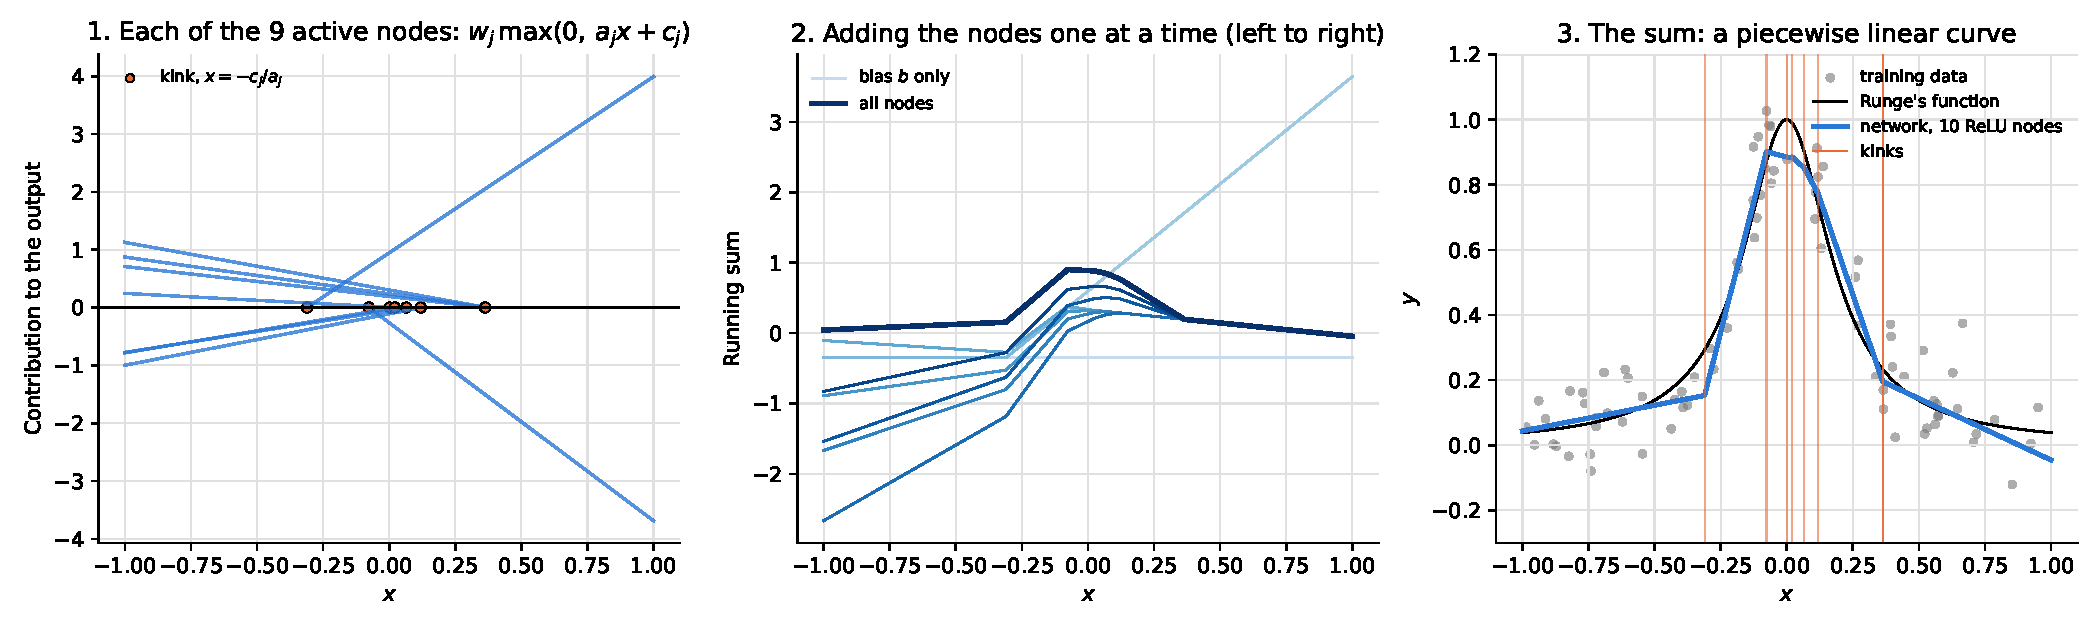
\includegraphics[width=\textwidth]{illustration_relu_hinges.pdf}
    \caption{How a network with one hidden layer of ten ReLU nodes builds its output, trained on the 80 training points of seed 42 (Adam, $\gamma = 3\times10^{-3}$, 4000 epochs). (1) The contribution $w_j\max(0, a_jx + c_j)$ of each node, with its kink at $x = -c_j/a_j$; one node is inactive on the whole interval and not shown. (2) The output bias, and the nodes added one at a time in the order of their kinks. (3) The sum, which is the output of the network, with the kinks marked.}
    \label{fig:hinges}
\end{figure*}

\emph{Learning rates.} Figure~\ref{fig:b_lr} shows the validation MSE after 1000 epochs for one hidden layer of 50 sigmoid nodes. SGD with RMSprop or Adam is best at $\gamma = 10^{-3}$ (0.0065 and 0.0062), below OLS of degree 12 (0.0112) on the same 16 points. Plain GD needs $\gamma = 0.1$ to get down to 0.0137, and blows up at $\gamma = 1$. For smaller $\gamma$ it stays at 0.08--0.10, about the variance of the validation targets (0.079), which is the error of the best constant prediction: the training has hardly started. The factor of 100 between the best learning rates comes from the division by $\sqrt{s}$. RMSprop and Adam take steps of about $\gamma$ for every weight, while GD takes $\gamma$ times the gradient, and the gradients here are small. For large $\gamma$ RMSprop and Adam get worse again, since steps of size $\gamma$ become too coarse. Adam is the least sensitive to $\gamma$, as in Project 1.

\begin{figure}
    \centering
    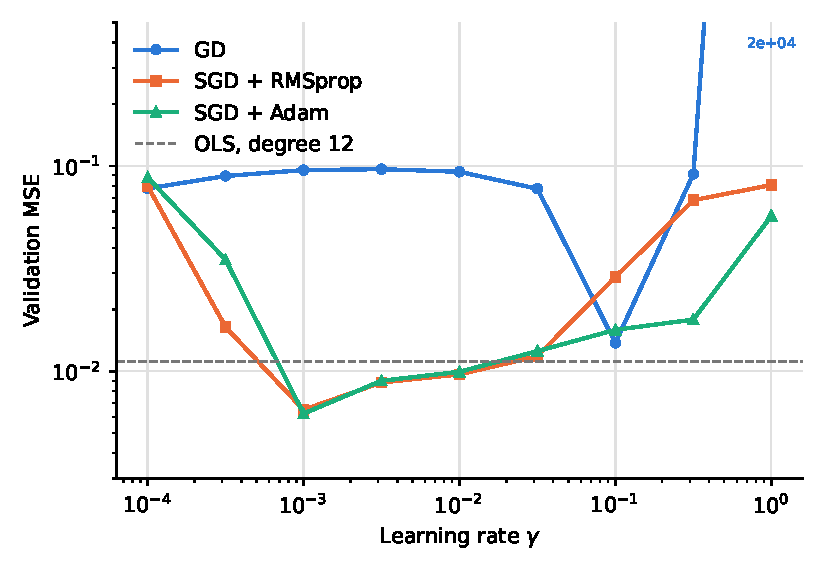
\includegraphics[width=\linewidth]{b_learning_rates.pdf}
    \caption{Validation MSE after 1000 epochs against the learning rate, one hidden layer of 50 sigmoid nodes, trained on 64 points of the seed-42 data set and validated on 16. GD uses all 64 points in each step, SGD minibatches of 16. The number at the top right is the MSE of GD at $\gamma = 1$. Dashed line: OLS of degree 12 fitted to the same 64 points.}
    \label{fig:b_lr}
\end{figure}

\emph{Training curves.} In Fig.~\ref{fig:b_curves} the MSE of GD with $\gamma = 0.1$ first grows to about 200 in six epochs and then falls back. The steps are too long for the curvature of the cost at the start, and in this run the weights moved after a few epochs to where the same step is stable. All three methods then stay on a plateau at about 0.1 for a long time before the MSE falls towards the noise level $\sigma^2 = 0.01$. After 1000 epochs the training MSE is 0.013--0.014 for the SGD methods and 0.030 for GD.

\begin{figure}
    \centering
    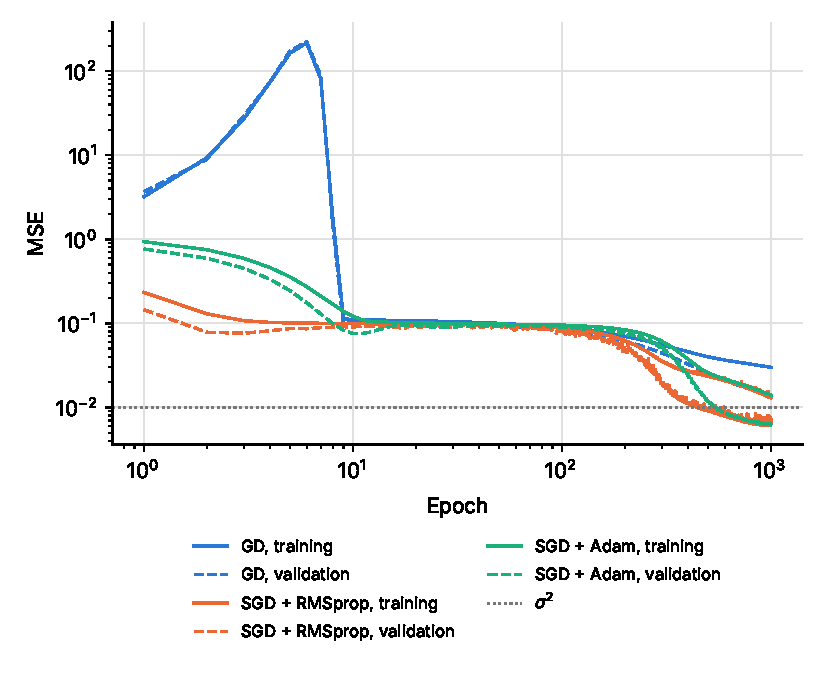
\includegraphics[width=\linewidth]{b_training_curves.pdf}
    \caption{Training (solid) and validation (dashed) MSE after each epoch for the three methods at their best learning rates (GD: $\gamma = 0.1$, RMSprop and Adam: $\gamma = 10^{-3}$), one hidden layer of 50 sigmoid nodes, seed 42. Dotted line: $\sigma^2$.}
    \label{fig:b_curves}
\end{figure}

The validation MSE ends lower than the training MSE, 0.0065 against 0.013 for RMSprop. This is chance in a small validation set: only 3 of the 16 validation points lie near the peak ($|x| < 0.2$), where the fit is hardest, against 18 of the 64 training points, and their noise happens to be smaller (mean squared noise 0.0090 against 0.0103).

\emph{More epochs.} GD is slower, not worse: after 3000 epochs it reaches 0.0068, where RMSprop and Adam were after 1000. Trained longer, RMSprop and Adam get worse (0.0097 and 0.0089 after 3000 epochs), and so does GD after $10\,000$ epochs (0.0101), as the network starts to follow the noise. The number of epochs thus works as a regularisation, like early stopping \cite[Sec.~8.12]{HjorthJensen2026}. The same number of epochs means the same cost, one pass through the data per epoch, but not the same number of updates: SGD makes four per epoch, GD one.

\emph{Architectures.} Table~\ref{tab:b_test} gives the test MSE on the seed-42 split for one and two hidden layers of 50 and 100 nodes, trained on all 80 training points. Only Adam beats OLS (0.0086), with 100 nodes or two layers, and only by a little. GD is clearly worse for all four architectures, but its learning rate was chosen for 50 nodes. None of the 20 test points lie near the peak, so the table mostly measures the flanks.

\begin{table}
    \centering
    \caption{Test MSE on the seed-42 split (20 test points), trained on all 80 training points for 1000 epochs, each method at the learning rate chosen in Fig.~\ref{fig:b_lr}. OLS of degree 12 on the same split: 0.0086.}
    \label{tab:b_test}
    \begin{tabular}{lcccc}
        \toprule
        Hidden layers & Parameters & GD & RMSprop & Adam \\
        \midrule
        50       & 151   & 0.0236 & 0.0123 & 0.0101 \\
        100      & 301   & 0.0651 & 0.0154 & 0.0083 \\
        50, 50   & 2701  & 0.0540 & 0.0111 & 0.0074 \\
        100, 100 & 10401 & 0.0572 & 0.0104 & 0.0078 \\
        \bottomrule
    \end{tabular}
\end{table}

In Fig.~\ref{fig:b_fits} the networks are smoother than the polynomial and do not reach the top of the peak. The polynomial wiggles along the flanks and shoots up above 1 beyond the last training point, at $x = 0.951$. Outside the data a polynomial of high degree cannot be trusted.

\begin{figure}
    \centering
    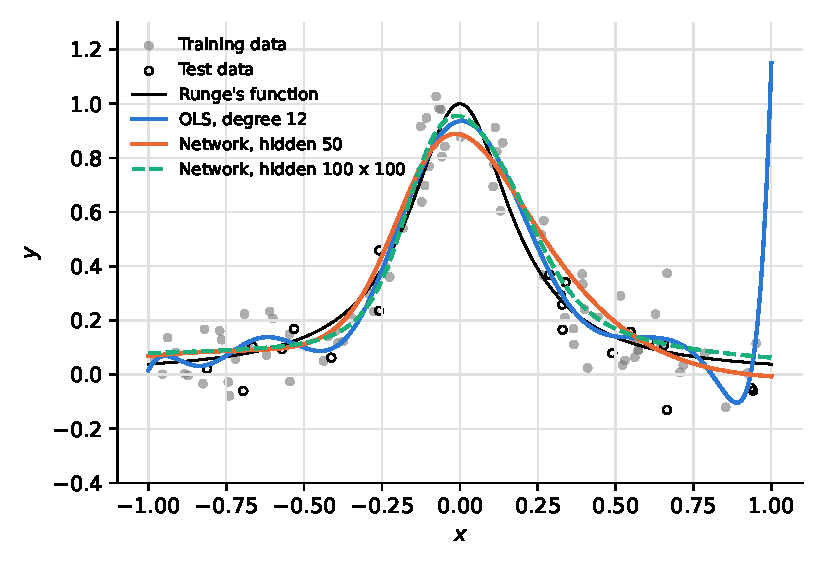
\includegraphics[width=\linewidth]{b_fits.pdf}
    \caption{The seed-42 data, Runge's function, OLS of degree 12 and two sigmoid networks trained with SGD and RMSprop on all 80 training points: one hidden layer of 50 nodes, and two hidden layers of 100 nodes.}
    \label{fig:b_fits}
\end{figure}

\emph{Several data sets.} Over ten data sets (seeds 42--51), with 50 nodes and RMSprop, the median test MSE was 0.0122 for OLS (25th--75th percentile 0.0095--0.0140) and 0.0132 for the network (0.0121--0.0160), and the network was better in only one of the ten. Here OLS of degree 12 is at least as good as the network, and it is a closed-form solution, while the network needs a learning rate, a number of epochs and a random initialisation.

\subsection*{Part c: activation functions, depth and width}

Figure~\ref{fig:c_heat} shows the median validation MSE for 1--5 hidden layers of 5--100 nodes, trained with Adam, $\gamma = 10^{-3}$. The best cells are 0.0125 for the sigmoid (five layers of 10 nodes), 0.0124 for ReLU (two of 10) and 0.0120 for Leaky ReLU (three of 5), and OLS gives 0.0119. Each validation MSE has a standard error of 20--30\,\% (Methods), so most of the differences between the cells are not significant. The sigmoid needs depth: with one hidden layer it stays at 0.017--0.023, and its worst cell, five layers of five nodes (0.068), has a median training MSE of 0.072, so it has hardly started to fit. For ReLU and Leaky ReLU the error is highest with five layers.

\begin{figure*}
    \centering
    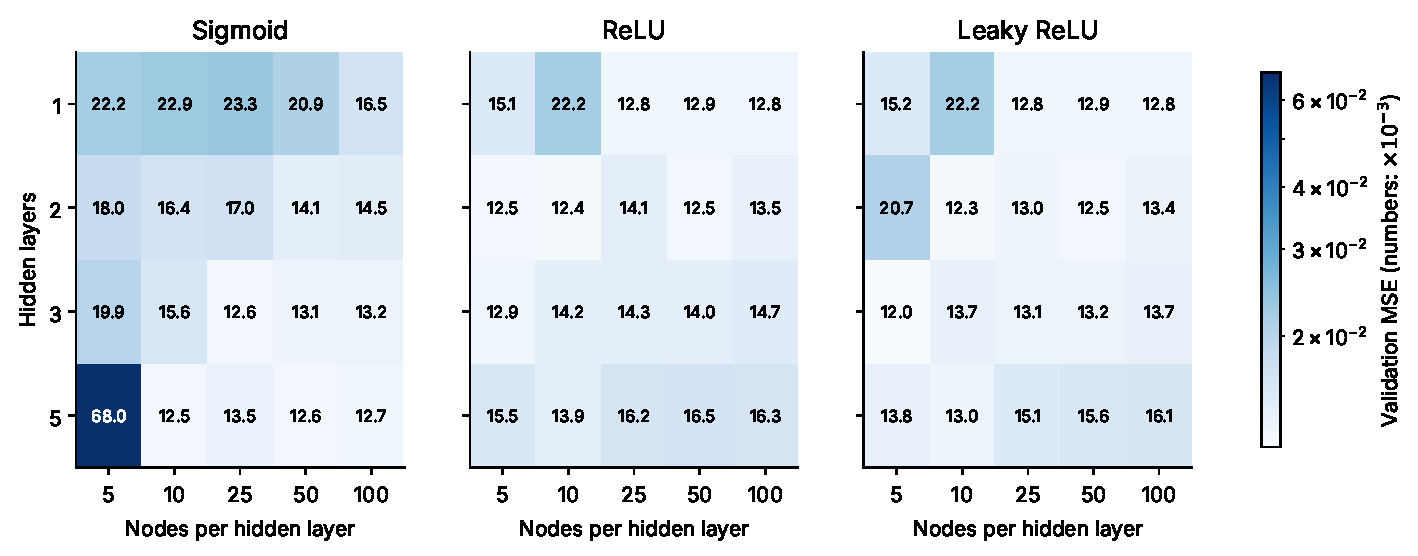
\includegraphics[width=0.9\textwidth]{c_heatmaps.pdf}
    \caption{Median validation MSE over three data sets (seeds 42--44) against the number of hidden layers and of nodes per layer, for sigmoid, ReLU and Leaky ReLU hidden layers; SGD with Adam, $\gamma = 10^{-3}$, minibatches of 16, 1000 epochs. The numbers are the MSE in units of $10^{-3}$, and lighter is better. OLS of degree 12 gives 11.9 on the same validation sets.}
    \label{fig:c_heat}
\end{figure*}

\emph{Overfitting.} In Fig.~\ref{fig:c_over}, with 50 nodes per layer, the training MSE of ReLU and Leaky ReLU falls below $\sigma^2$ as layers are added (about 0.0074 with three and five layers), while the validation MSE grows from 0.0125 with two layers to 0.0165 and 0.0156 with five. With up to $10\,351$ parameters for 64 training points, the networks follow the noise. This is overfitting, as for a high polynomial degree in Project 1. For the sigmoid both curves keep falling, since it learns more slowly. Trained for 5000 epochs instead of 1000, the sigmoid network with five layers reaches a training MSE of 0.0078 and a validation MSE of 0.0144 (0.0085 and 0.0126 after 1000), so it overfits too, only later.

\begin{figure}
    \centering
    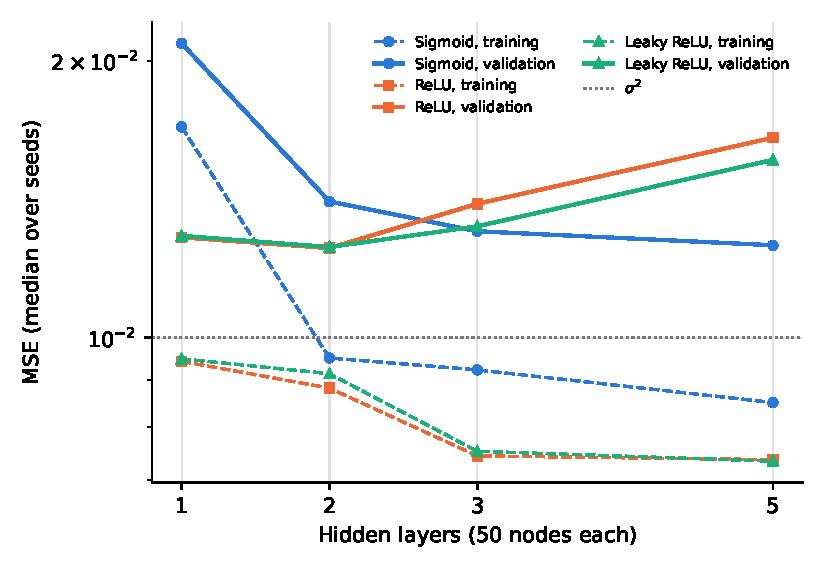
\includegraphics[width=\linewidth]{c_overfitting.pdf}
    \caption{Training (dashed) and validation (solid) MSE against the number of hidden layers of 50 nodes, median over seeds 42--44, from the same runs as Fig.~\ref{fig:c_heat}. Dotted line: $\sigma^2$.}
    \label{fig:c_over}
\end{figure}

\emph{Vanishing gradients.} Figure~\ref{fig:c_grad} shows the root mean square of the weight gradient in each layer of a network with five hidden layers of 50 nodes. For the sigmoid at initialisation it falls from 0.79 in the output layer to $10^{-5}$ in the first hidden layer, by a factor of about 4--5 per layer in the middle of the network. Each layer on the way back multiplies $\boldsymbol{\delta}$ by the transposed weights and by $\sigma'(z) \le 1/4$, so the gradient shrinks geometrically towards the input \cite[Sec.~8.9]{HjorthJensen2026}. With ReLU, whose derivative is 1 for active nodes, and He initialisation, it is 0.1--0.2 in all hidden layers. After 100 epochs the sigmoid gradients in the hidden layers are still about 6 to 50 times smaller than the ReLU gradients, which fits with the sigmoid needing more epochs. We used the root mean square per weight, and not the norm of the whole matrix as in Fig.~8.14 of the lecture notes, because the first and the last layer have 50 weights and the others 2500, and the norm grows with the number of weights.

\begin{figure*}
    \centering
    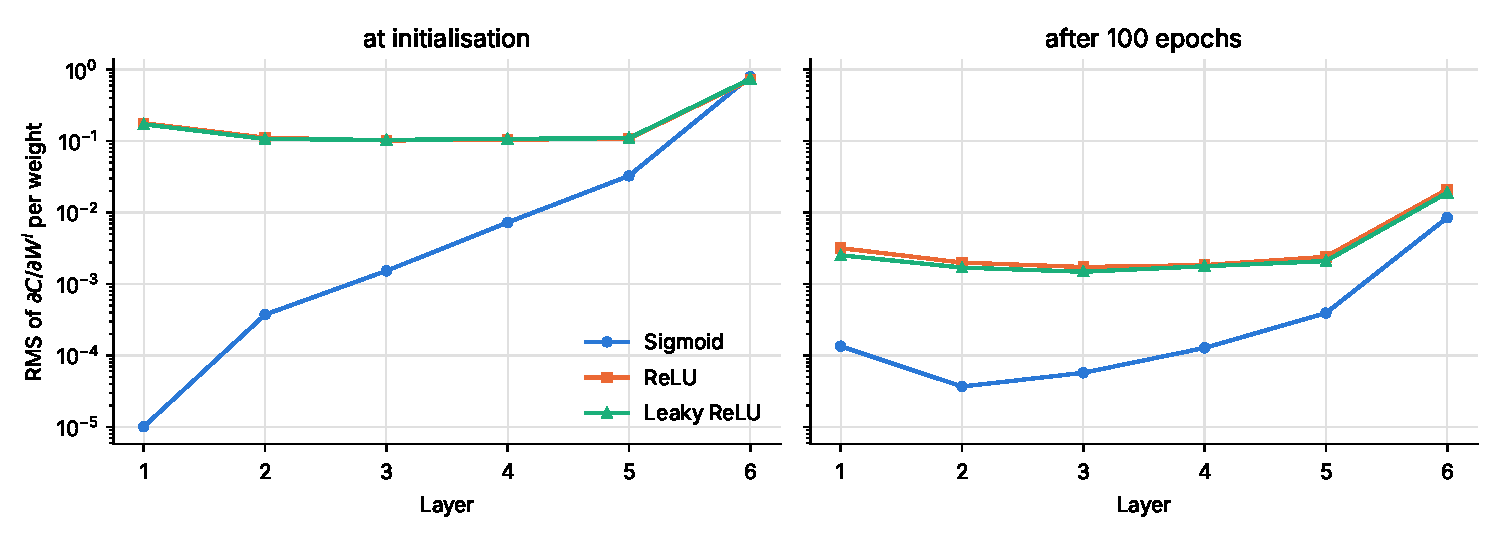
\includegraphics[width=0.85\textwidth]{c_gradient_norms.pdf}
    \caption{Root mean square of $\partial C/\partial \mathbf{W}^l$ over the weights of each layer, for a network with five hidden layers of 50 nodes (layer 1: first hidden layer, layer 6: output layer), on the 64 training points of seed 42. Left: at initialisation. Right: after 100 epochs with Adam, $\gamma = 10^{-3}$.}
    \label{fig:c_grad}
\end{figure*}

\emph{Which activation?} For this problem the three activations reach the same level in their best configurations. The sigmoid needs more layers or more epochs, because its gradients vanish towards the input. ReLU and Leaky ReLU learn faster, but overfit when the network gets deep. Leaky ReLU, which cannot have completely dead nodes, gave practically the same results as ReLU.

\subsection*{Part d: $L_1$ and $L_2$ penalties}

For the penalties we used the ReLU network with three hidden layers of 50 nodes, which overfits in part c. In Fig.~\ref{fig:d_heat} the best cell for $L_2$ has $\lambda = 0$ (0.0123), and the best for $L_1$ has $\lambda = 10^{-6}$ (0.0120), which is no real difference. $\lambda = 10^{-2}$ is clearly worse (0.015--0.027): it pulls the weights so hard that the network can no longer follow the function, as a large $\lambda$ did in Ridge and Lasso. Both grids are best at the smallest learning rate, $\gamma = 10^{-4}$, at the edge of the grid. With this $\gamma$ the network does not get far enough in 1000 epochs to follow the noise, so the learning rate and the fixed number of epochs already regularise the network, and the penalty has little left to do. At larger $\gamma$ moderate penalties do somewhat better than $\lambda = 0$, for instance 0.0127 against 0.0140 for $L_2$ with $\lambda = 10^{-4}$ at $\gamma = 10^{-3}$, but within the uncertainty.

\begin{figure*}
    \centering
    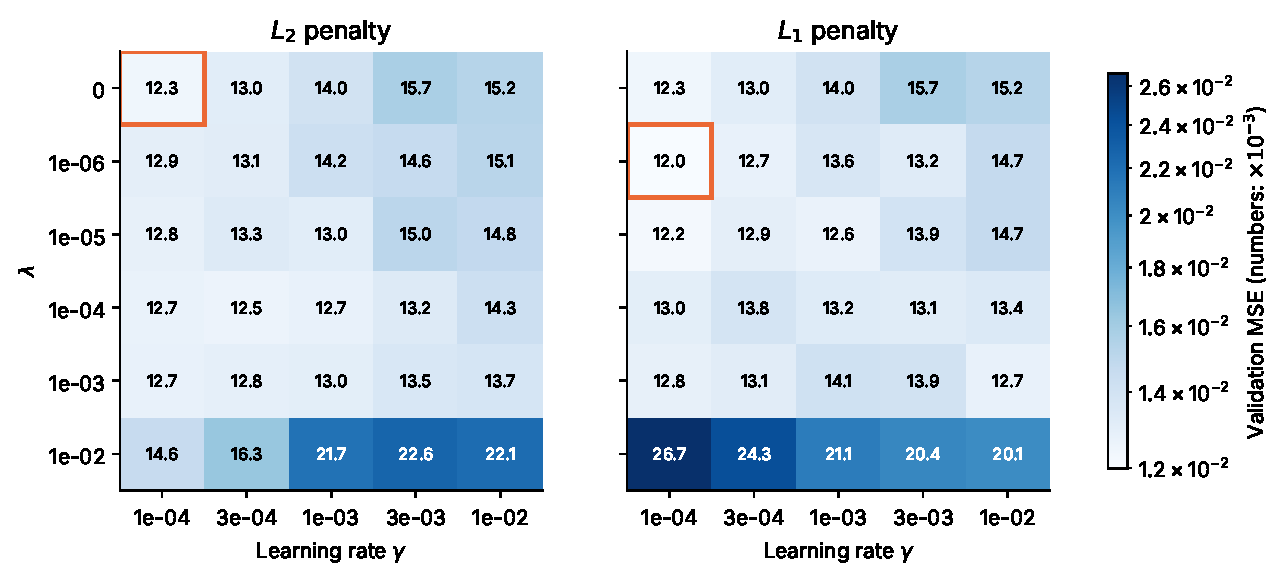
\includegraphics[width=0.8\textwidth]{d_heatmaps.pdf}
    \caption{Median validation MSE over seeds 42--44 against the learning rate $\gamma$ and the penalty $\lambda$, for the $L_2$ (left) and $L_1$ (right) penalty; three hidden layers of 50 ReLU nodes, Adam, minibatches of 16, 1000 epochs. The numbers are the MSE in units of $10^{-3}$, and the orange square marks the lowest value. The row $\lambda = 0$ is the same in both panels.}
    \label{fig:d_heat}
\end{figure*}

Table~\ref{tab:d_test} gives the test MSE on the 20 data sets of Project 1. Since $\lambda = 0$ was best for $L_2$, the $L_2$ network is the network without penalty. Its median, 0.0093, is lower than for Ridge (0.0133), Lasso (0.0139) and OLS (0.0155), and close to the median mean squared noise of 0.0091, which is what even the true function gets. Its 75th percentile (0.0116) is below the median of Ridge. The hyperparameters were chosen on the validation sets of seeds 42--44, so the test sets played no part in the choice.

\begin{table}
    \centering
    \caption{Test MSE on the 20 data sets of Project 1 (seeds 42--61): median and 25th--75th percentile over the data sets. Networks: three hidden layers of 50 ReLU nodes, Adam, $\gamma = 10^{-4}$, 1000 epochs on all 80 training points. Project 1: degree and $\lambda$ chosen by 5-fold cross-validation. Noise: the mean squared noise $(y_i - f(x_i))^2$ in the test sets.}
    \label{tab:d_test}
    \begin{tabular}{lcc}
        \toprule
        Model & Median & Percentiles \\
        \midrule
        Network, no penalty                 & 0.0093 & 0.0084--0.0116 \\
        Network, $L_1$, $\lambda = 10^{-6}$ & 0.0096 & 0.0083--0.0119 \\
        OLS (Project 1)                     & 0.0155 & -- \\
        Ridge (Project 1)                   & 0.0133 & -- \\
        Lasso (Project 1)                   & 0.0139 & -- \\
        Noise                               & 0.0091 & -- \\
        \bottomrule
    \end{tabular}
\end{table}

So the penalty is not why the network beats Ridge and Lasso. In Project 1 the largest errors of the polynomials came from data sets where they had to extrapolate or bridge a gap near the edges of the interval. The ReLU network continues as a straight line outside its outermost kinks and cannot oscillate like a polynomial of high degree, so it avoids these errors. In Project 1, Ridge improved on OLS by keeping the high-degree polynomials from blowing up; for the network, the small learning rate already prevents overfitting. The Lasso solver of Project 1 did not converge for the small $\lambda$ chosen by cross-validation, so the Lasso numbers are approximate. The network also differs from the one in part b in the activation, the depth, the optimiser and the learning rate, and we did not test which of these made it better than OLS.

\subsection*{Part e: classification of MNIST}

All the MNIST networks have 784 inputs, a softmax output layer of 10 nodes and the cross entropy as cost, and were trained with Adam in minibatches of 128 for 20 epochs, with the $L_2$ penalty.

\emph{Learning rate and penalty.} In Fig.~\ref{fig:e_heat}, for one hidden layer of 100 ReLU nodes, the best combination is $\gamma = 10^{-3}$ and $\lambda = 10^{-5}$ (0.9783), but for $\lambda \le 10^{-4}$ the differences are within the standard error of 0.0014. $\lambda = 10^{-3}$ is too strong (0.9640 at $\gamma = 10^{-3}$), $\gamma = 10^{-4}$ is too slow for 20 epochs (about 0.95), and $\gamma = 3\times10^{-3}$ is a little worse than $10^{-3}$. As for the Runge data, the penalty gave no measurable gain. The validation accuracy (Fig.~\ref{fig:e_curves}) flattens out at about 0.98 after ten epochs without a downward trend, so there is no clear overfitting for the penalty to remove.

\begin{figure}
    \centering
    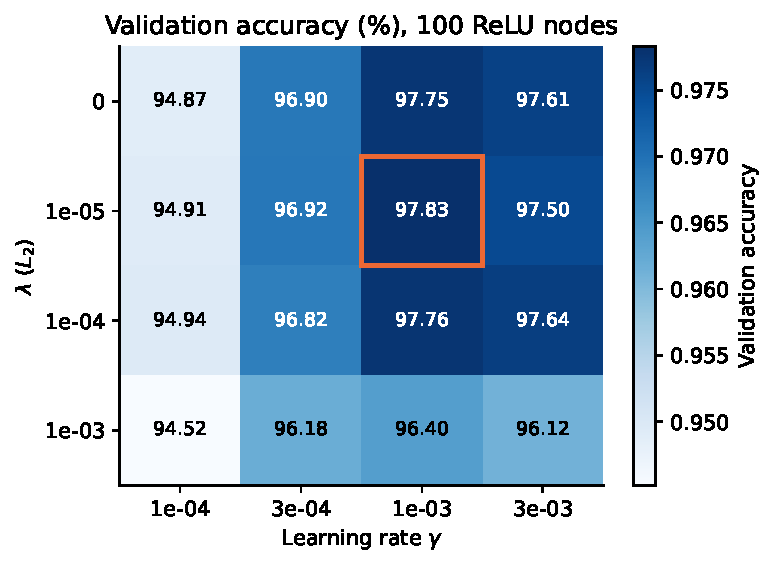
\includegraphics[width=0.9\linewidth]{e_heatmap.pdf}
    \caption{Validation accuracy in percent on MNIST against the learning rate $\gamma$ and the $L_2$ penalty $\lambda$; one hidden layer of 100 ReLU nodes, Adam, minibatches of 128, 20 epochs. The orange square marks the best value. The standard error of each number is about 0.14 percentage points.}
    \label{fig:e_heat}
\end{figure}

\begin{figure}
    \centering
    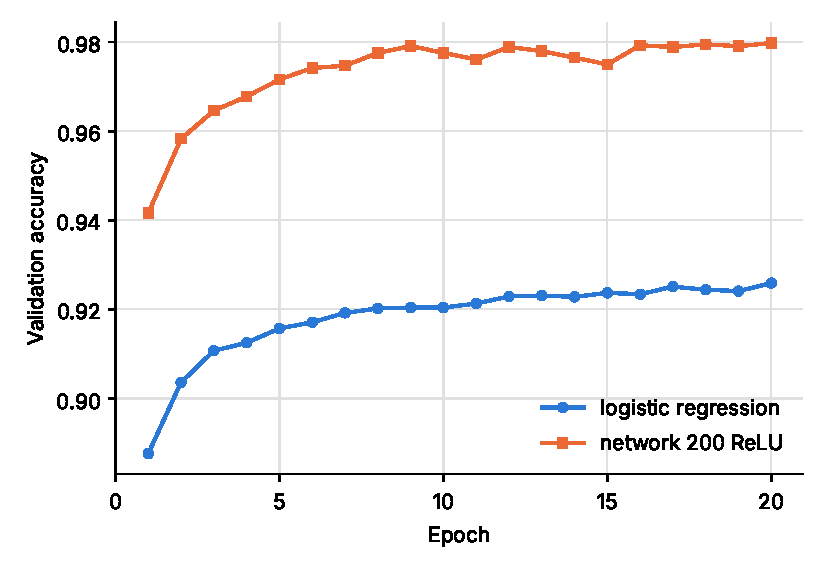
\includegraphics[width=\linewidth]{e_training_curves.pdf}
    \caption{Validation accuracy after each epoch for logistic regression ($\gamma = 10^{-3}$) and for the network with one hidden layer of 200 ReLU nodes ($\gamma = 10^{-3}$, $\lambda = 10^{-5}$).}
    \label{fig:e_curves}
\end{figure}

\emph{Architecture and activation.} In Table~\ref{tab:e_arch}, wider is better up to 200 nodes, and two layers of 100 nodes are not better than one layer of 200. ReLU and Leaky ReLU are equal, and the sigmoid is 0.2--0.5 percentage points lower. We chose one hidden layer of 200 ReLU nodes (0.9798), but Leaky ReLU with 200 nodes (0.9795) is within the standard error. A single run also depends on chance in the training. With other seeds for the initial weights and the minibatch order, the same network reached 0.9798, 0.9795 and 0.9703 after 20 epochs. The low value is a dip in the last epoch; one epoch earlier that run was at 0.9795. With a constant learning rate Adam does not settle at a minimum, and over the last ten epochs each of the three runs varied by 0.35 to 0.92 percentage points. Differences of a few tenths of a percentage point between the cells are therefore not meaningful.

\begin{table}
    \centering
    \caption{Validation accuracy on MNIST for different hidden layers and activations, at $\gamma = 10^{-3}$ and $\lambda = 10^{-5}$, after 20 epochs. The standard error is about 0.0014.}
    \label{tab:e_arch}
    \begin{tabular}{lcccc}
        \toprule
        Activation & 50 & 100 & 200 & 100, 100 \\
        \midrule
        Sigmoid    & 0.9633 & 0.9730 & 0.9762 & 0.9753 \\
        ReLU       & 0.9669 & 0.9783 & 0.9798 & 0.9773 \\
        Leaky ReLU & 0.9684 & 0.9783 & 0.9795 & 0.9769 \\
        \bottomrule
    \end{tabular}
\end{table}

\emph{Test results.} The test set was used once, for the chosen network, for logistic regression at its best learning rate ($\gamma = 10^{-3}$) and for the scikit-learn models:

\noindent\begin{minipage}{\linewidth}
\begin{lstlisting}[style=terminal]
Test set (10000 images), used once
  most frequent digit              accuracy 0.1135
  logistic regression              accuracy 0.9273 +- 0.0026
  network 200 ReLU                 accuracy 0.9777 +- 0.0015
  scikit-learn LogisticRegression  accuracy 0.9245
  scikit-learn MLPClassifier       accuracy 0.9797
\end{lstlisting}
\end{minipage}

The network makes 223 errors on the $10\,000$ test images, against 727 for logistic regression, 69\,\% fewer. scikit-learn gets nearly the same accuracies with the same models, which supports our implementation; its network also differs from ours in the initialisation and the penalty. Logistic regression on raw pixels is known to give about 92\,\%, and convolutional networks above 99\,\% \cite{LeCun1998}. The network took about eight times longer to train than logistic regression (74\,s against 9\,s on our machine).

\emph{Why the hidden layer helps.} Logistic regression computes one score per digit, a weighted sum over the pixels $p$,
$$
z_k = \sum_{p} w_{pk}\,x_p + b_k ,
$$
so the weights of digit $k$ form a $28\times28$ template (top row of Fig.~\ref{fig:weights}). The score is high when the image has ink where the template is positive (red) and none where it is negative (blue). The templates are blurred, since each of them must match every way of writing its digit. The hidden nodes (lower rows) do not belong to any digit. They respond to parts of digits, such as strokes in certain places, and the output layer combines them. More weights alone would not help: with a linear activation in the hidden layer, the network would still be a linear function of the pixels. It is the non-linear activation that lets the network combine features, for instance to recognise different ways of writing the same digit, which one linear template per digit cannot.

\begin{figure*}
    \centering
    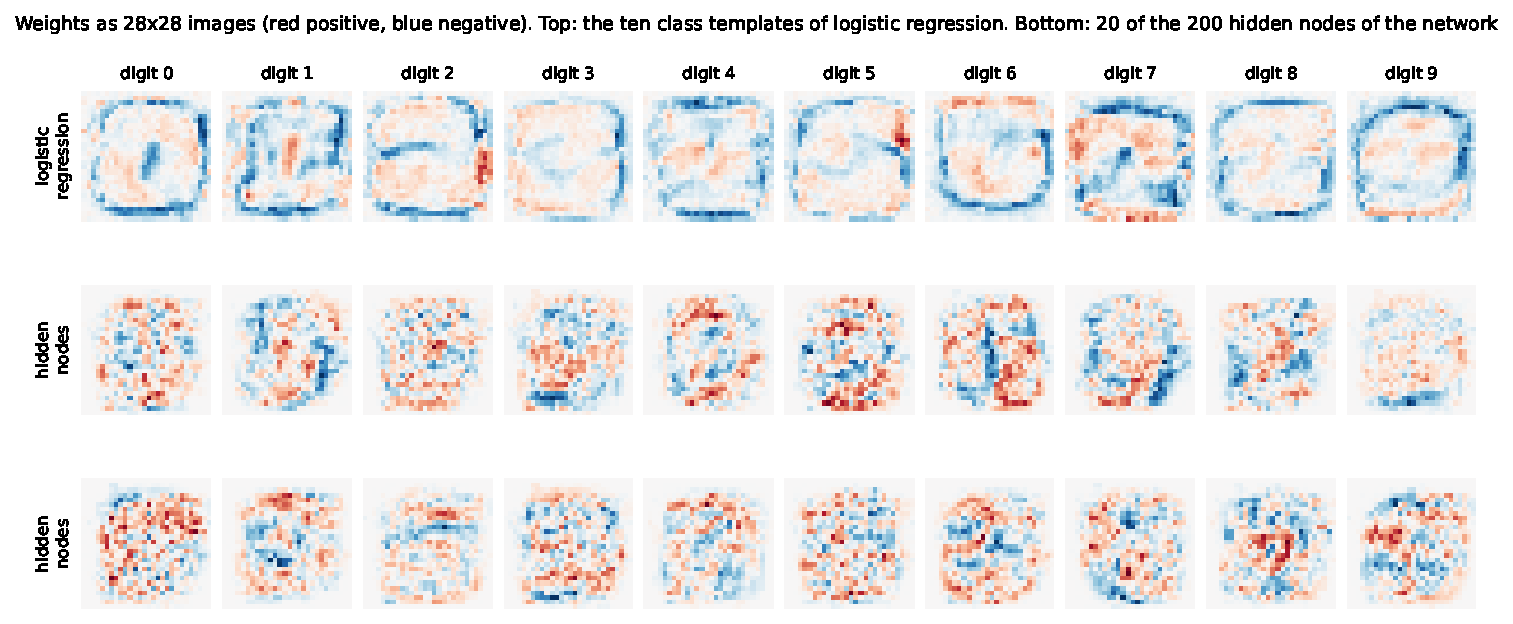
\includegraphics[width=0.85\textwidth]{illustration_mnist_weights.pdf}
    \caption{The weights from the 784 pixels shown as $28\times28$ images (red positive, blue negative, each image on its own colour scale). Top row: the ten digit templates of logistic regression. Lower rows: the weights into 20 of the 200 hidden nodes of the network, chosen at random.}
    \label{fig:weights}
\end{figure*}

\emph{Which errors remain?} The errors in Fig.~\ref{fig:e_conf} are concentrated in pairs of digits that can look alike: 2 classified as 8 (14 images), 4 as 9 (14), 9 as 7 (8), 2 as 7 (8), and 5 as 6 and as 3 (7 each). The precision is lowest for 8 (0.954), so other digits are often classified as 8, and the recall is lowest for 2 (0.961) and 9 (0.967), so these are most often classified as something else. The network reduced the errors most for the digits that logistic regression found hardest: 5 (from 116 to 25), 2 (109 to 40), 9 (100 to 33), 8 (95 to 23) and 3 (81 to 19). The accuracy alone shows none of this.

\begin{figure*}
    \centering
    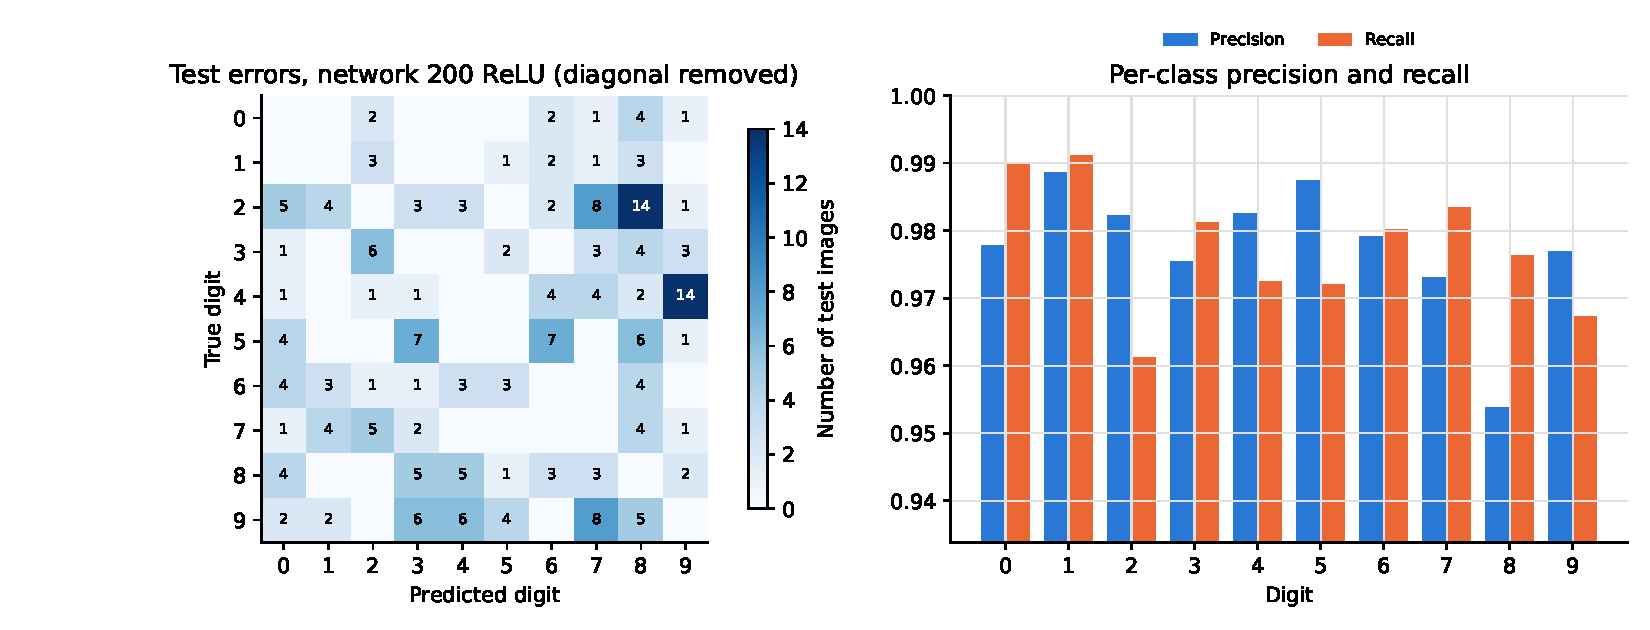
\includegraphics[width=0.85\textwidth]{e_confusion.pdf}
    \caption{Left: the confusion matrix of the network with 200 ReLU nodes on the $10\,000$ test images, with the diagonal (the correct answers) removed so that the errors are visible. Right: precision and recall for each digit.}
    \label{fig:e_conf}
\end{figure*}

% =====================================================================
% CRITICAL EVALUATION (part f)
% LLM declaration: text level 3; see the appendix "Use of AI/LLM tools".
% =====================================================================

\section*{Critical evaluation}

\emph{Regression.} OLS has a closed-form solution. It takes milliseconds, gives the same result every time and needs no learning rate, and with a good degree it was as good as our first networks. But we must choose the features ourselves, a polynomial of high degree oscillates near the edges and blows up outside the data (Fig.~\ref{fig:b_fits}), and the best degree depends on the data set. Ridge keeps the high degrees under control with a small penalty, still in closed form, and was the best method in Project 1. Lasso has no closed form, and its solver was slow and did not always converge. The network learns its features from $x$ alone, and the ReLU network gave the lowest test error of all the methods, close to the noise level, mainly by doing better near the edges. On the other hand it has many hyperparameters (architecture, activation, optimiser, learning rate, minibatch size, number of epochs and penalty), its cost is not convex, so the result depends on the initial weights and the minibatches, and it trains in seconds instead of milliseconds. With only 16 validation points the choice of hyperparameters was noisy, and $k$-fold cross-validation on the 80 training points, as in Project 1, would have used the data better. For a smooth function of one variable, OLS or Ridge is the natural first choice. The network pays off when the function is hard to describe with a polynomial, as near the edges here.

\emph{Classification.} Logistic regression has a convex cost with one minimum, few hyperparameters and short training, and its weights can be read as templates. It is the baseline a network must beat. The network with one hidden layer beat it clearly, with 69\,\% fewer errors, because the features that make up a handwritten digit are not known in advance, and the hidden layer, with its non-linear activation, learns them. This is where the network earns its extra cost, about ten times the training time and more hyperparameters. Of the methods we tried, it is the best for the classification; convolutional networks do better still.

\emph{Gradient methods.} Plain gradient descent has only one parameter, $\gamma$, but its step is proportional to the gradient. It needed a learning rate 100 times larger than RMSprop and Adam, overshot at the start and converged slowly, and its best $\gamma$ changes with the architecture. RMSprop and Adam scale each step to about $\gamma$, so $\gamma = 10^{-3}$ worked well for all the architectures and on both data sets, and with minibatches they make several updates per epoch. Adam was the least sensitive to $\gamma$, and we used it for parts c--e. With a constant learning rate and a fixed number of epochs, when to stop matters: trained longer, the networks started to follow the noise, and on MNIST the accuracy jumped from epoch to epoch.

% =====================================================================
% CONCLUSION
% LLM declaration: text level 3; see the appendix "Use of AI/LLM tools".
% =====================================================================

\section*{Conclusion}

We wrote a feed-forward neural network with backpropagation and checked it against automatic differentiation and the closed-form OLS solution. On Runge's function, one hidden layer of 50 sigmoid nodes was not better than OLS of degree 12, with a median test MSE over ten data sets of 0.0132 against 0.0122. A ReLU network with three hidden layers of 50 nodes, trained with Adam and a small learning rate, reached 0.0093 on the 20 data sets of Project 1, against 0.0133 for Ridge and close to the noise level of 0.0091, mainly by doing better near the edges. The ReLU networks overfitted with depth and the sigmoid networks with more epochs; the sigmoid gradients vanish towards the input by a factor of about 4--5 per layer. The $L_1$ and $L_2$ penalties gave no measurable improvement, since the small learning rate and the fixed number of epochs already prevented overfitting. RMSprop and Adam needed a learning rate 100 times smaller than plain gradient descent and reached low errors in fewer epochs. On MNIST, one hidden layer of 200 ReLU nodes gave a test accuracy of 97.8\,\%, against 92.7\,\% for logistic regression, and most of the remaining errors were between digits that can look alike, such as 4 and 9.

The Runge validation and test sets are small, so most differences between architectures and penalties are within the uncertainty. We used a fixed number of epochs, coarse grids and, on MNIST, single runs, whose accuracy varied by up to almost one percentage point between epochs. Cross-validation, early stopping on the validation set and averages over several runs would make the comparisons more reliable.

% =====================================================================
% APPENDIX: declaration of AI/LLM use
% =====================================================================

\appendix

\section*{Appendix: Use of AI/LLM tools}

\paragraph*{Tools used.} Claude (Opus 5.5), used through claude.ai with its code-execution workspace, October 2026. Claude was also used as a tutor for the theory and for the weekly exercises of weeks 41--43; the understanding this gave is not declared separately.

\paragraph*{Text.} Contribution levels as defined in the course guidelines.

\begin{center}
    \begin{tabular}{lc}
        \toprule
        Section & Level \\
        \midrule
        Abstract & 3 \\
        Introduction & 3 \\
        Methods & 3 \\
        Results and discussion & 3 \\
        Critical evaluation & 3 \\
        Conclusion & 3 \\
        Appendix (this declaration) & 3 \\
        \bottomrule
    \end{tabular}
\end{center}

\emph{Level 3 note.} All sections were drafted by Claude from our dialogue during the project. For each part we first gave our own answers to the questions in the project text and our own reading of the figures and the logged output, and Claude corrected them. The prompt for the draft was to write the report from this dialogue, to include only what we had shown that we understand, and to take every number from the logged output of the code; Claude then checked the numbers in the text against the logs. \textcolor{red}{[To be completed after revision: the main changes we made to the draft.]}

\paragraph*{Code.} Contribution levels as defined in the course guidelines. Every file has an \texttt{LLM-assisted} note at the top that covers all its functions, and the larger functions carry a short tag that refers to it.

\begin{center}
    \begin{tabular}{lcp{0.62\linewidth}}
        \toprule
        File & Level & Description \\
        \midrule
        \texttt{nn.py} & 4 & Activations, costs, the network class and the training loop, written by Claude. The backpropagation (\texttt{compute\_gradient}) is our own batched backpropagation from the week 42 exercises, moved into the class by Claude, who added the output error for the cross entropies and the penalty terms. \\
        \texttt{main.py} & 4 & One function per project part, the figures and the logged output, written by Claude from the experiments we agreed on, including the two illustrations (Figs.~\ref{fig:hinges} and \ref{fig:weights}), which we asked for. \\
        \texttt{tests.py} & 4 & The two tests, written by Claude; the checks are the ones the project text asks for. \\
        \texttt{optim.py} & 4 & Update rules from Project 1, unchanged. \\
        \texttt{common.py} & 4 & Data, design matrix, scaling and OLS from Project 1, unchanged. \\
        \bottomrule
    \end{tabular}
\end{center}

The results in this report were produced by running the code locally on a Windows machine. The choices behind the experiments (data sets, seeds, validation split, grids and what to compare with) were discussed and agreed on before the code was written.


\bibliographystyle{apsrev4-1}
\bibliography{refs}
\end{document}
